\section{Anwendung des Kalman-Filters}
\subsection{Ziel}
Bis jetzt haben wir gelesen, was das Kalman-Filter bewirkt und wie es funktioniert.
Nun möchten wir mit einem Beispiel herausfinden, ob das Filter unsere gesuchte Grösse $f(t)$ bestimmen kann

\subsection{Künstliche Erdbebendaten}
Da wir keine Rohdaten über vergangene Erdbeben zur Hand haben, müssen wir mittels Matlab künstliche Daten erzeugen und sie dann in das Filter eingeben.
Diese Vorgehensweise erlaubt uns das Erdbeben beliebig zu gestalten und weil es digital simuliert wird, haben wir keine Bauschäden zu beklagen.

\subsection{Wahl der Schwingung}
Wir müssen uns überlegen, mit welcher Schwingung wir ein realitätsnahes Beben erzeugen können.

Mit einer ungedämpften harmonischen Schwingung können wir zwar die meisten Vorgänge in der Physik erklären.
Da aber unser Erdbeben irgendwann abklingen muss, wählen wir die gedämpfte harmonische Schwingung.
Die dazugehörige Schwingungsgleichung lautet

\begin{equation}
	y = A \sin(\omega t e^{-\lambda t})
\end{equation} 

Für die Variablen der harmonisch gedämpften Schwingung setzen wir die Werte

\begin{equation}
A = 5
\end{equation} 

ein.

$A$ ist die Amplitude der Schwingung, die uns die Heftigkeit des Erdebebens beschreibt.
Sie ist vergleichbar mit der Magnitude.

$\omega$ definiert sich durch 

\begin{equation}
	\omega = 2 \pi f
\end{equation}

wobei die Frequenz f mit

\begin{equation}
	f = E(Frequenz) + \sigma^2(Frequenz)
\end{equation}

erzeugt wird.

Zusätzlich haben wir $f$ mit dem Savitzky-Golay-Filter gefiltert.
Das Savitzky-Golay-Filter schaut sich immer eine definierte Anzahl von Datenpunkte an und bildet ein Polygon n-ter Ordnung. 
In unserer Anwendung schaut sich das Filter, im Sinne eines verschieblichen Fensters, jeweils zehn aufeinanderfolgende Datenpunkte an und bildet ein Polygon 0-ter Ordnung. 
Da wir den Grad 0 gewählt haben, erhalten wir pro zehn Punkte nur eine Gerade mit der Steigung 0. 
Diese Art von Mittelwertbildung nennt sich auch moving average oder auf Deutsch gleitender Mittelwert.

Für den Erwartungswert und die Standardabweichung setzen wir die Zahlen 

\begin{equation}
E(f) = 15 Hz
\end{equation}

und 
\begin{equation}
\sigma^2 = 10 Hz
\end{equation}

ein.

$\lambda$ ist die Bodendämpfung, für die wir 0.2 wählen.
Sie ist dafür verantwortlich, dass unser Erdbeben abklingen wird und kreiert bei der gedämpften Schwingung die typische Hüllkurve der Amplitude.
Wir nehmen an, dass $\lambda$ ein Materialparameter von geologischen Böden ist.

\subsection{Ab hier bin ich noch dran/ Versuch im Standardfall}
Im nächsten Schritt müssen wir sinnvolle Systemparameter für unseren Seismographen definieren.
Eine kurze Recherche zeigt, dass die Masse ein Gewicht von ca. 100 g hat.
Da wir das Erdbeben nach Augenmass realistisch darstellen möchten, geben wir der realistischen Masse eher weniger Gewichtung und definieren $m = 0.01$
Zur Federkonstante D und Dämpfung k konnten wir leider keine brauchbaren Grössen finden und treffen die Annahme, dass $D = 1$ und $k = 0.01$.

Da unser Seismograph von der Umgebung durch Wind, Temperatur oder menschgemachten Vibrationen beeinflusst wird, müssen wir ein Prozessrauschen definieren.
Die dazugehörige Matrix $Q$ beinhaltet die Standardabweichung für die Position, Geschwindigkeit und äussere Kraft.
Wir nehmen an, dass

\begin{equation}
	Q = \left(
	\begin{array}{ccc} 	
		{\sigma_x }^2& 0& 0 \\ 
		0 & {\sigma_v }^2& 0\\ 
		0 & 0& {\sigma_f }^2\\
	\end{array}\right)= \left(
	\begin{array}{ccc} 	
		{0.00001 }^2& 0& 0 \\ 
		0 & {0.00001 }^2& 0\\ 
		0 & 0& {1 }^2\\
	\end{array}\right)
\end{equation} 

Auch für die Messung setzen wir ein Rauschen voraus und definieren

\begin{equation}
R= ({\sigma_x}^2)=
({0.00001}^2)
\end{equation}

Sind nun die benötigten Systemparameter und das Rauschen definiert, erzeugen wir das Erdbeben und schauen wie gut das Kalman-Filter die äussere Beschleunigung schätzen kann.

Wie wir in Abbildung 20.4 sehen, liegen wir mit unseren definierten Werten ziemlich gut.
Das Positions-Zeit-Diagramm stellt eine realistische Erdbebenschwingung auf.
Das Ziel, ein künstliches Erdbeben zu kreieren haben wir somit erreicht.
Nun möchten wir noch herausfinden, ob auch das Kalman-Filter eine gute Schätzung hervorbringen konnte.
Wir betrachten in Abbildung 20.5 das vergrösserte Kraft-Zeit-Diagramm und erkennen, dass die Schätzung sehr nahe an die Erdbebenschwingung kommt.

\begin{figure}
	\begin{center}
		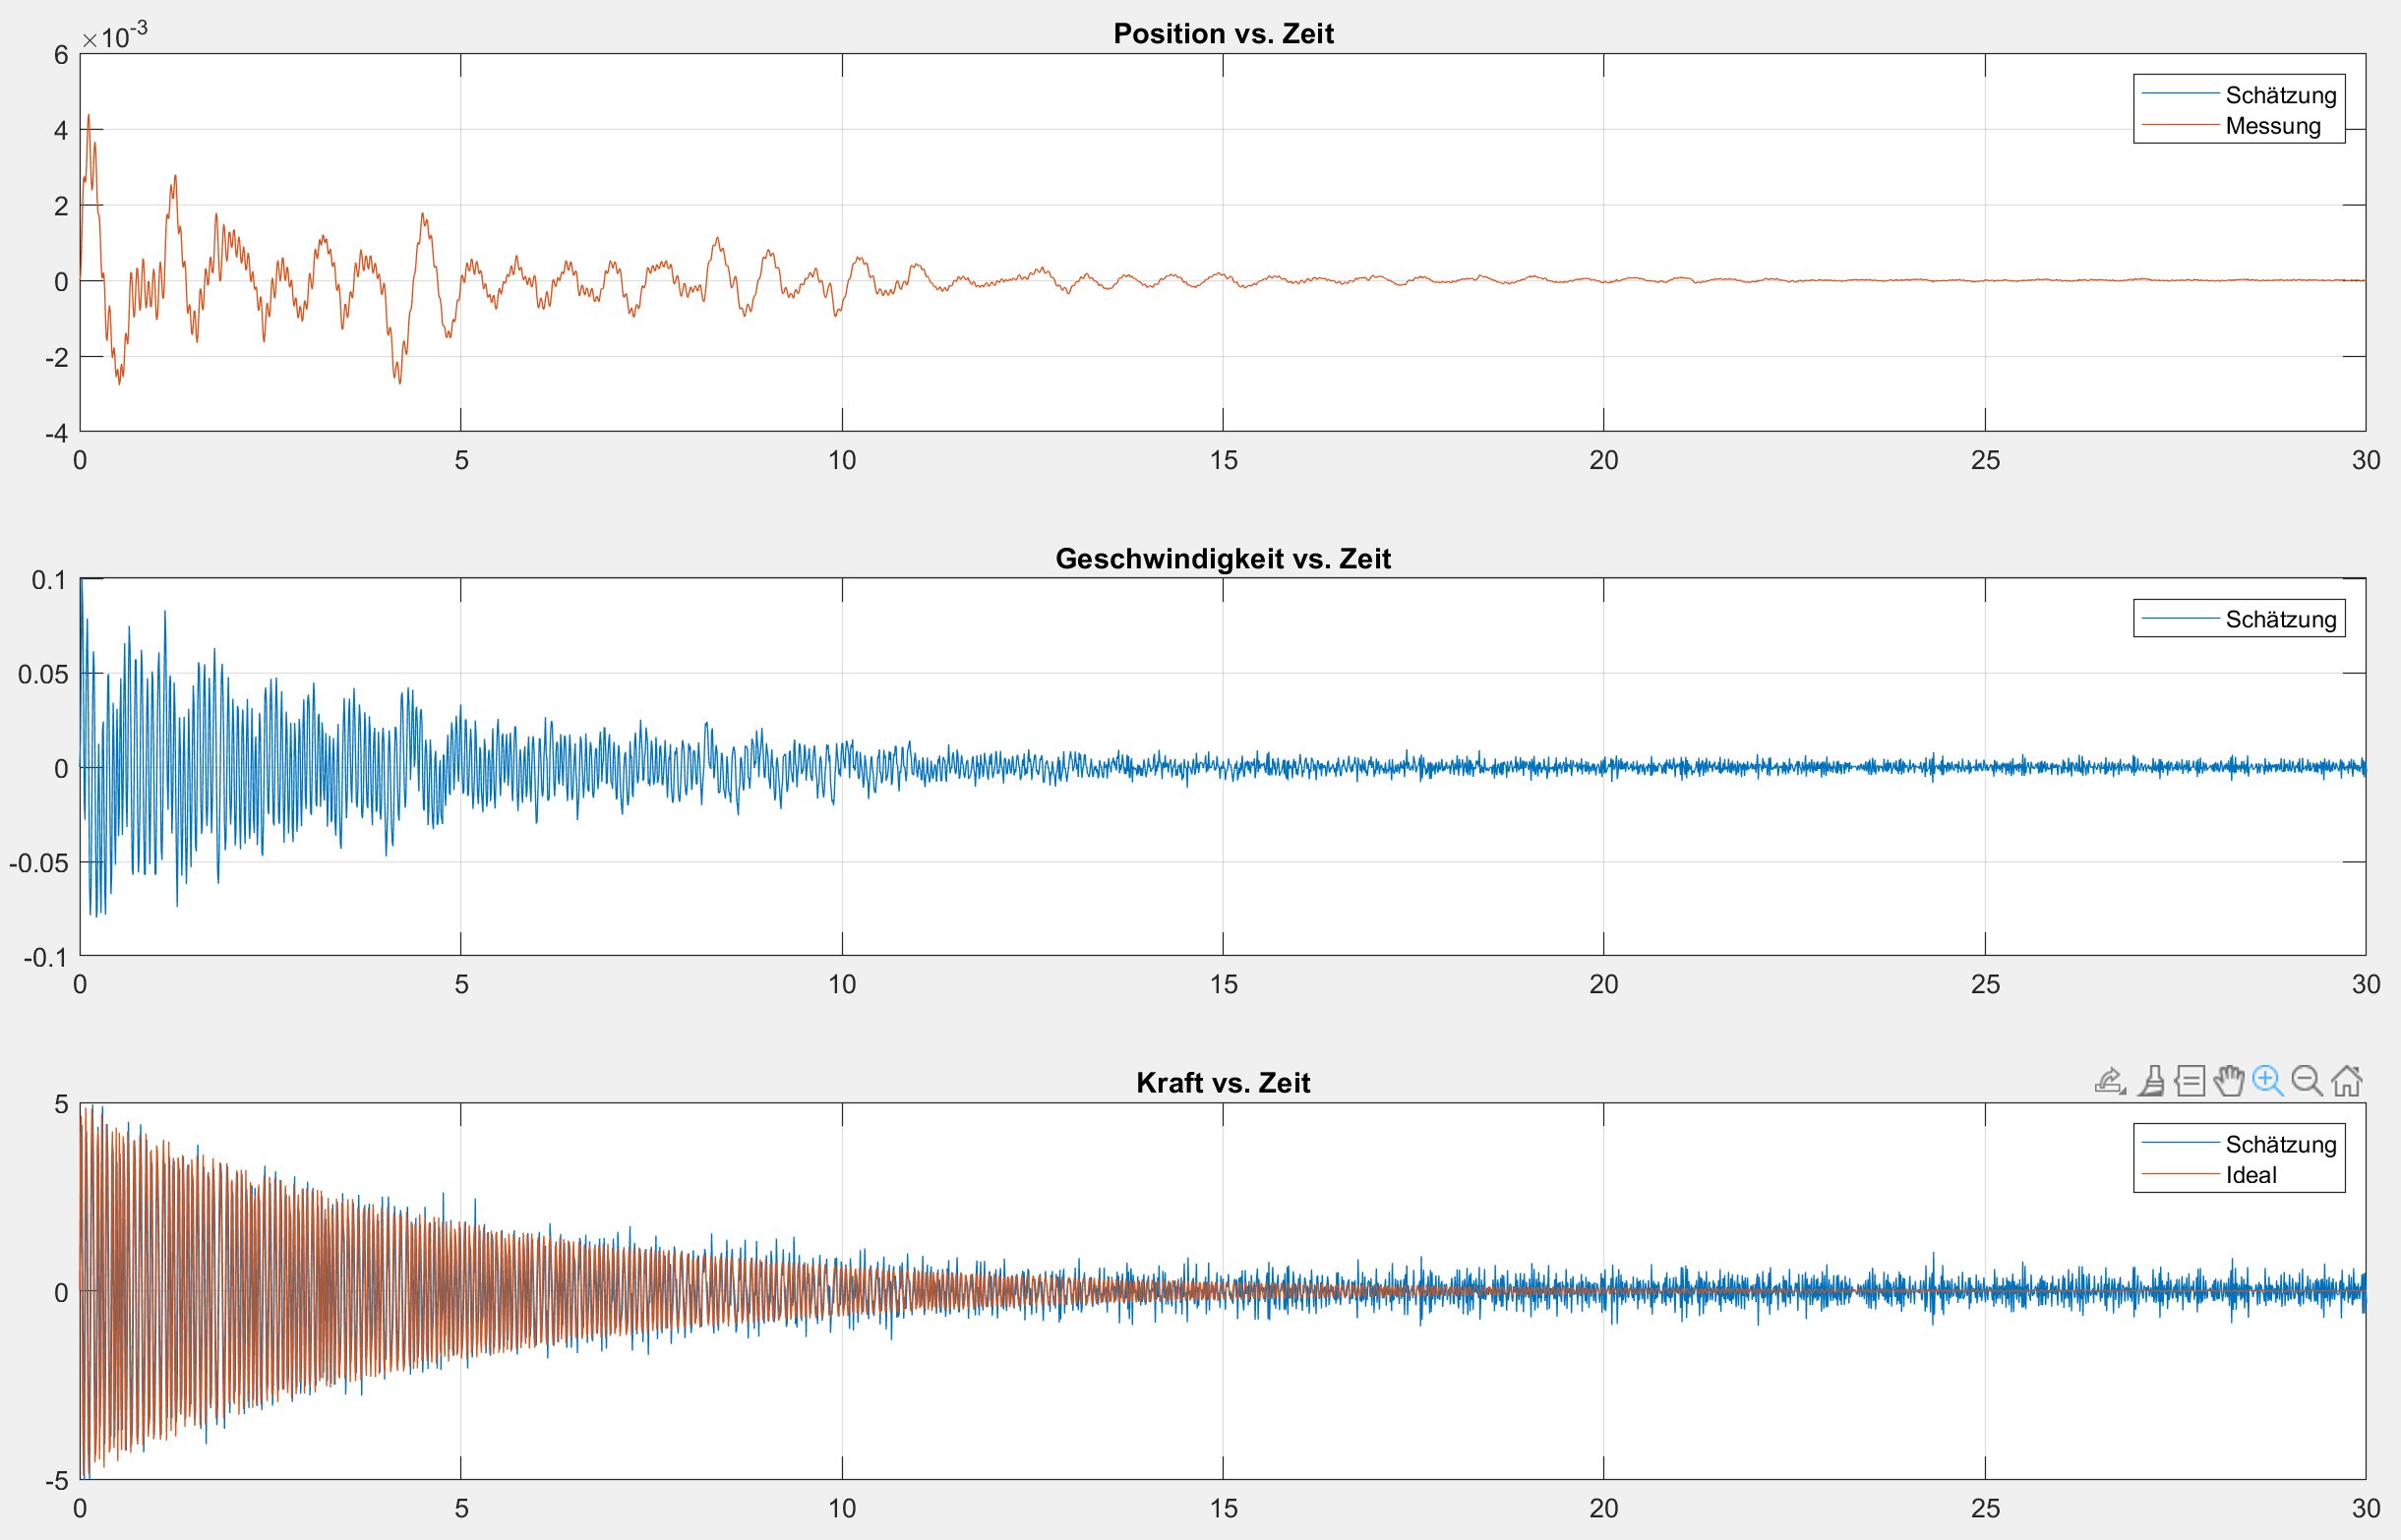
\includegraphics[width=15cm]{papers/erdbeben/Standard_alles.PNG}
		\caption{Die Grafik Position vs. Zeit zeigt die typische Aufzeichnung eines Erdbebens. In der Grafik Kraft vs. Zeit wird unteranderem die äussere Beschleunigung mittels Kalman Filters bestimmt.}
	\end{center}
\end{figure}

\begin{figure}
	\begin{center}
		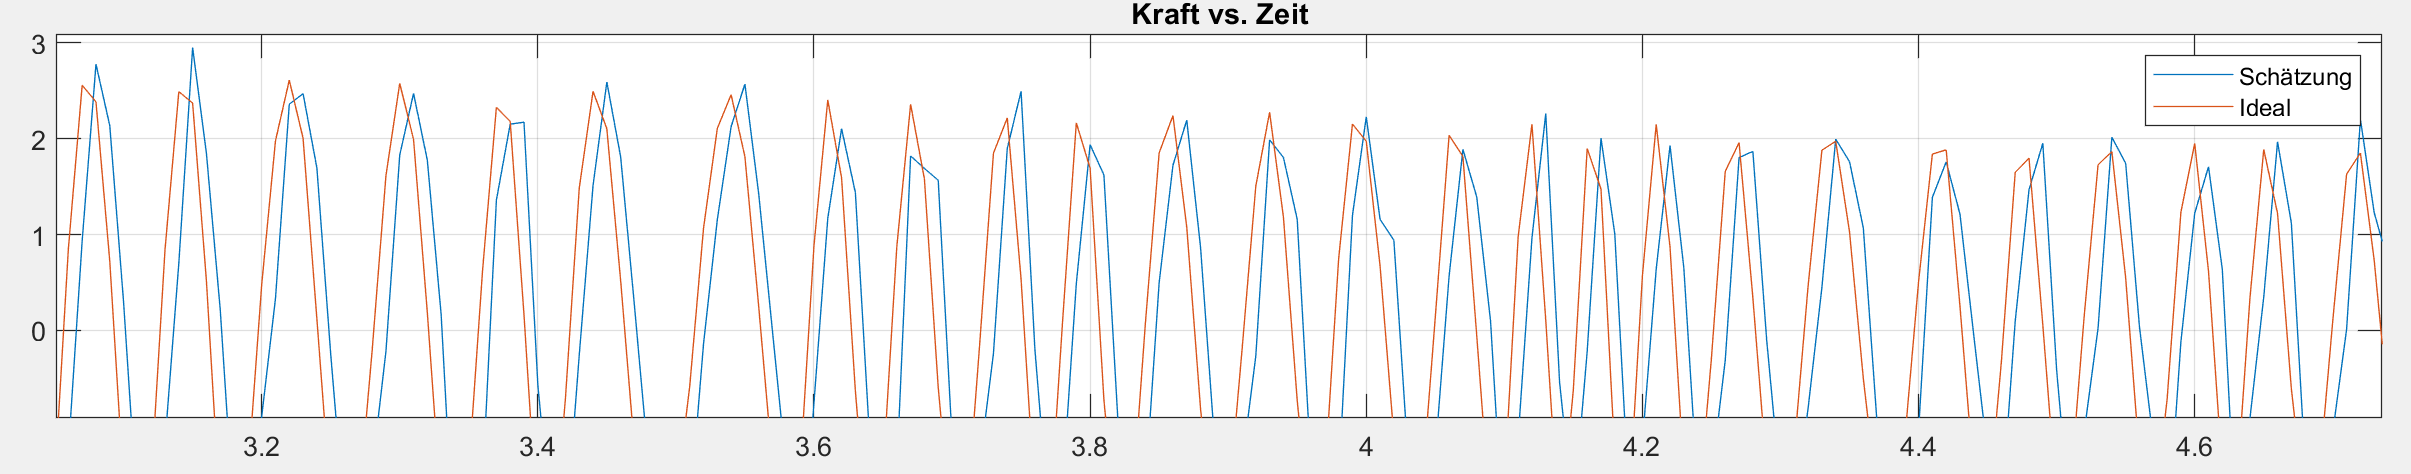
\includegraphics[width=15cm]{papers/erdbeben/Erdbeben_Standardfall_Zoom.PNG}
		\caption{Erst das Vergrössern des Diagrammes zeigt uns auf, wie gut die Schätzung des Kalman-Filters funktioniert.}
	\end{center}
\end{figure}

Wir können nun an den Systemparametern Werte verändern oder das Rauschen des Prozesses und der Messung verstärken.

\subsection{Veränderung der Systemparameter}




\subsection{Verstärkung des Prozessrauschens}
Vertrauen wir dem Seismographen weniger als beim Standardfall, erhöhen wir das Prozessrauschen.
Mit der Erhöhung des Rauschens teilen wir dem Filter mit, dass wir 

Gründe dafür könnten den Standort oder die Bauweise des Seismographen sein.
Seismographen sind meistens an Orten verbaut, wo es aus der Umgebung wenig Einflüsse gibt.
Steht der Seismograph in der Nähe einer grösseren Stadt, werden viel mehr Vibrationen aufgezeichnet, die aber nicht von einem Erdbeben stammen und somit die Aufzeichnung verfälschen.
Auch die Qualität des Seismographen spielt eine Rolle, wie genau die Position oder Geschwindigkeit aufgezeichnet wird.

Wir verstärken das Prozessrauschen um den Faktor 10'000 aber belassen den Rest gleich wie beim Standardfall.
Wir erwarten nun, dass die Geschwindigkeit und Position der Masse verrauschter und somit unkenntlicher erfasst wird.

Das Seismogramm zeichnet nun 
Wir erwarten, dass die Aufzeichnung der Position und Geschwindigkeit ungenauer wird, 

\begin{figure}
	\begin{center}
		\includegraphics[width=15cm]{papers/erdbeben/Prozessrauschen_geändert.PNG}
		\caption{Das verstärkte Rauschen dominiert über der Erdbebenschwingung. Die Aufzeichnung wird unbrauchbar.}
	\end{center}
\end{figure}

\subsection{Verstärkung des Messrauschens}




\subsection{Fazit}
Grafik einfügen
Wir erkennen, dass wir mit dem Kalman-Filter eine gute Methode gefunden haben, die äussere Beschleunigung zu schätzen. Die Schätzung der nächsten Position der Federmasse liegt immer ziemlich nahe der tatsächlichen Messung. Man muss aber auch berücksichtigen, dass die Federschwingung ziemlich kontrolliert verläuft und das Kalman-Filter somit präzise Vorhersagen treffen kann.
